\documentclass[tikz,border=2pt]{standalone}
\usepackage[T1]{fontenc}
\usepackage{libertine}
\usepackage{xcolor}
\usetikzlibrary{arrows.meta,positioning}

\begin{document}
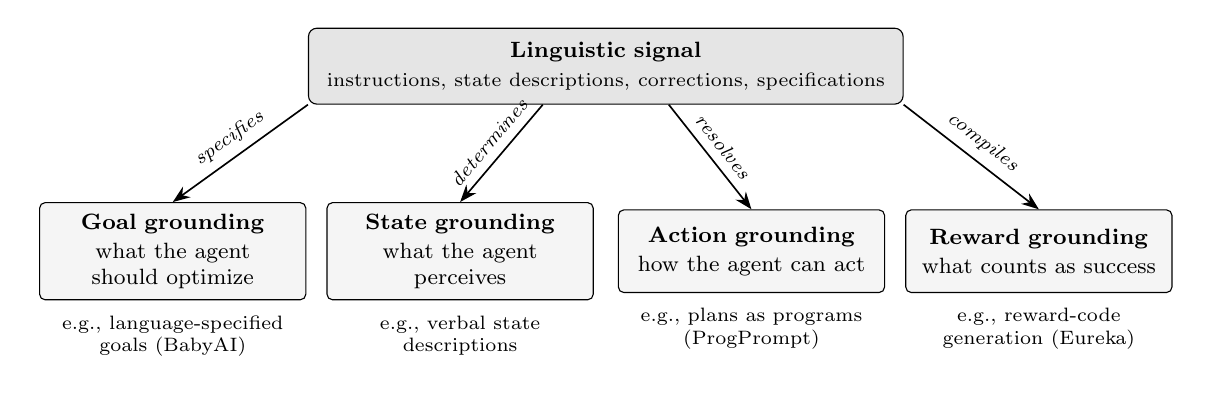
\begin{tikzpicture}[
    font=\footnotesize,
    source/.style={draw, rounded corners=3pt, fill=gray!20, align=center,
        inner sep=5pt, text width=7.2cm},
    component/.style={draw, rounded corners=2pt, fill=gray!8, align=center,
        inner sep=4pt, text width=3.1cm, minimum height=1.05cm},
    exemplar/.style={align=center, text width=3.45cm, font=\scriptsize},
    map/.style={-{Stealth[length=2.2mm]}, semithick},
]
    \node[source] (signal) at (0, 2.35)
        {\textbf{Linguistic signal}\\[1pt]
         {\scriptsize instructions, state descriptions, corrections, specifications}};
    \node[component] (goal) at (-5.5, 0)
        {\textbf{Goal grounding}\\[1pt] what the agent should optimize};
    \node[component] (state) at (-1.85, 0)
        {\textbf{State grounding}\\[1pt] what the agent perceives};
    \node[component] (action) at (1.85, 0)
        {\textbf{Action grounding}\\[1pt] how the agent can act};
    \node[component] (reward) at (5.5, 0)
        {\textbf{Reward grounding}\\[1pt] what counts as success};
    \node[exemplar, below=2pt of goal] {e.g., language-specified\\ goals (BabyAI)};
    \node[exemplar, below=2pt of state] {e.g., verbal state\\ descriptions};
    \node[exemplar, below=2pt of action] {e.g., plans as programs\\ (ProgPrompt)};
    \node[exemplar, below=2pt of reward] {e.g., reward-code\\ generation (Eureka)};
    \draw[map] (signal.south west) to node[midway, sloped, above, font=\scriptsize\itshape] {specifies} (goal.north);
    \draw[map] ([xshift=-0.8cm]signal.south) to node[midway, sloped, above, font=\scriptsize\itshape] {determines} (state.north);
    \draw[map] ([xshift=0.8cm]signal.south) to node[midway, sloped, above, font=\scriptsize\itshape] {resolves} (action.north);
    \draw[map] (signal.south east) to node[midway, sloped, above, font=\scriptsize\itshape] {compiles} (reward.north);
\end{tikzpicture}
\end{document}
